\subsection*{Partie I : Théorème du point fixe}
Dans tout le problème, on dira que $x$ est un point fixe de $g$ si et seulement si $g(x)=x$.
\begin{enumerate}
 \item 
\begin{enumerate}
 \item 
On suppose que $g$ est $k$-lipschitzienne dans $I$.\newline
Pour tout $x\in I$ et tout $\varepsilon>0$, en prenant $\alpha = \frac{\varepsilon}{k}$, on a :
\begin{displaymath}
 |y-x|< \alpha \Rightarrow |g(y)-g(x)|\leq k |y-x|= \varepsilon
\end{displaymath}
Ce qui montre que $g$ est continue en $x$. On remarque que le $\alpha$ est le même pour tous les $x$ de $I$ (uniforme continuité).

\item Montrons d'abord l'existence d'un point fixe. \newline Considérons la fonction définie dans $I$
\begin{displaymath}
 \varphi : x \rightarrow g(x) - x
\end{displaymath}
Elle est continue comme somme de deux fonctions continues. La stabilité de $I$ par $g$ entraîne que $g(a)\geq a$ donc $\varphi(a) \geq 0$ et que $g(b)\leq a$ donc $\varphi(b) \leq 0$. Lorsque l'une des deux inégalités est une égalité, $a$ ou $b$ est un point fixe. Lorsque les deux inégalités sont strictes, on peut appliquer le théorème des valeurs intermédiaires à $\varphi$ entre $a$ et $b$. Il existe donc un $x\in ]a,b[$ tel que $\varphi(x)=0$, c'est à dire un point fixe pour $g$.\newline
Montrons ensuite l'unicité d'un point fixe. Soit $x$ et $y$ deux points fixes :
\begin{displaymath}
 |x-y|=|g(x)-g(y)|\leq k |x-y|\Rightarrow (1-k)|x-y|\leq 0 \Rightarrow x=y
\end{displaymath}
car $1-k >0$ par hypothèse.\newline
On note $\alpha$ l'unique point fixe de $g$.
\end{enumerate}

\item
\begin{enumerate}
 \item On applique $n$ fois l'inégalité de lipschitzité :
\begin{multline*}
 |x_n - \alpha| = |g(x_{n-1} - g(\alpha)|\leq k |x_{n-1}-\alpha|=  k|g(x_{n-2} - g(\alpha)| \\ 
\leq k^2 |x_{n-2}-\alpha| \leq \cdots \leq  k^p |x_{n-p}-\alpha| \leq k^n |x_{0}-\alpha| = k^n|u-\alpha|
\end{multline*}
La suite à droite de l'inégalité précédente est géométrique de raison $k \in]0,1[$. Elle converge donc vers $0$ ce qui permet d'appliquer le théorème d'encadrement. La suite $(x_n)_{n\in \N}$ converge vers $\alpha$.
\item Utilisons d'abord l'inégalité triangulaire 
\begin{multline*}
 |x_{n+p}-x_n|\leq |x_{n+p}-x_{n+p-1}|+ |x_{n+p-1}-x_{n+p-2}|+ \cdots +|x_{n+1}-x_{n}|\\
=\sum_{i=0}^{p-1}|x_{n+1+i}-x_{n+i}|
\end{multline*}
puis majorons comme plus haut en utilisant le caractère lipschitzien
\begin{multline*}
 |x_{n+1+i}-x_{n+i}|=|g(x_{n+i})-g(x_{n+i-1})|\\
 \leq k |x_{n+i}-x_{n+i-1}| \leq \cdots \leq k^i |x_{n+1}-x_{n}|
\end{multline*}
En injectant dans la première majoration, on obtient :
\begin{displaymath}
 |x_{n+p}-x_n|\leq \left(\sum_{i=0}^{p-1}k^i\right) |x_{n+1}-x_{n}| = \frac{1-k^p}{1-k}|x_{n+1}-x_{n}|
\end{displaymath}

\item Dans l'inégalité précédente, fixons $n$ et considèrons les suites en $p$.\newline
La suite $(x_{n+p})_{p\in \N}$ converge vers  $\alpha$, la suite $(x_{n})_{p\in \N}$ est constante, la suite $(k^p)_{p\in \N}$ converge vers 0. Par opérations sur les suites convergentes et passage à la limite dans une inégalité, on obtient donc :
\begin{displaymath}
 |\alpha - x_n|\leq \frac{1}{1-k}|x_{n+1}-x_{n}|
\end{displaymath}
\end{enumerate}

\item \begin{enumerate}
 \item Comme $g$ est supposée dérivable en $\alpha$, on peut écrire :
\begin{displaymath}
 |g'(\alpha)| =  \lim_{h\rightarrow 0} \left|\frac{g(\alpha +h) -g(\alpha)}{h}\right|\leq k
\end{displaymath}
d'après l'inégalité de lipschitzité et le théorème de passage à la limite dans une inégalité.

\item Par définition de $x_n$ et comme $g(\alpha)=\alpha$ :
\begin{displaymath}
 \frac{x_{n+1}-\alpha}{x_n -\alpha}=\frac{g(x_n)-g(\alpha)}{x_n -\alpha} \rightarrow g'(\alpha)
\end{displaymath}
à cause de la dérivabilité en $\alpha$ car $(x_n)_{n\in \N}$ converge vers $\alpha$.
\end{enumerate}
\end{enumerate}

\subsection*{Partie II. Méthode de Newton}
\begin{enumerate}
 \item \begin{enumerate}
 \item L'équation considérée admet une solution à cause du théorème des valeurs intermédiaires appliqué à $f$ entre $a$ et $b$. Cette solution est unique car la fonction est strictement croissante à cause du signe de la dérivée. L'unique solution notée $\alpha$ sera appelée \emph{zéro} de $f$.
\item L'équation de la tangente en $x_0$ est :
\begin{displaymath}
 y = f'(x_0)(x-x_0)+f(x_0)
\end{displaymath}
L'abcisse du point d'intersection avec l'axe d'équation $y=0$ est
\begin{displaymath}
 x_0 - \frac{f(x_0)}{f'(x_0)}
\end{displaymath}
\end{enumerate}

\item 
\begin{enumerate}
 \item La fonction $f$ est $\mathcal C^2$ donc sa dérivée est $\mathcal C^1$. De plus $f$ est strictement positive ce qui assure le caractère $\mathcal C^1$ de l'inverse. Les résultats usuels sur les opérations sur les fonctions continues et dérivables montrent que $g$ est de classe $\mathcal C^1$. 
\item Comme $\alpha$ est un zéro de $f$:
\begin{displaymath}
 g(\alpha)=\alpha, \hspace{0.5cm} g'(\alpha) = 1 -1 +\frac{f(\alpha)f''(\alpha)}{f'(\alpha)^2} = 0
\end{displaymath}
On en déduit que $\alpha$ est à la fois un zéro de $f$ et un point fixe de $g$.
\end{enumerate}

\begin{figure}[h]
  \centering
  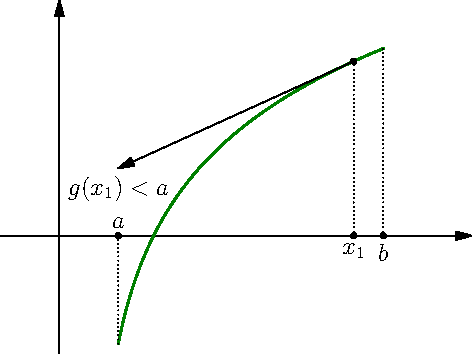
\includegraphics{./Cnewton_1.pdf}
  % Cnewton_1.pdf: 128x170 pixel, 72dpi, 4.52x6.00 cm, bb=0 0 128 170
  \caption{II.3.a. Exemple de graphe de $f$}
  \label{fig:Cnewton_1}
\end{figure}

\item \begin{enumerate}
 \item La restriction de $\ln$ à un segment de $]0,+\infty[$ satisfait aux conditions. Dans la Figure \ref{fig:Cnewton_1} on a tracé un graphe de ce genre.
 \item Remarquons que l'intervalle $[a,b]$ complet \emph{n'est pas stable}. On a indiqué sur la figure \ref{fig:Cnewton_1} un point $x_1$ dont l'image n'est pas dans $[a,b]$.\newline
 Montrons que l'intervalle $[a,\alpha]$ est stable.\newline
 Montrons d'abord que la restriction de $g$ est croissante. En effet:
\[
 g'(x) = \frac{f(x)f''(x)}{f'(x)^2} > 0
\]
car $f''$ est négative partout et $f(x)< 0$ dans $[a,\alpha[$. D'autre part $g(\alpha) > \alpha$ car $f(\alpha)<0$ donc 
\[
 g(\left[ a, \alpha\right]) = \left[ g(a), g(\alpha)\right] =   \left[ g(a), \alpha\right] \subset  \left[ a, \alpha\right].   
\]
On peut aussi remarquer (calcul de $g'$) que, dans $[a,\alpha]$, $g$ est croissante et telle que $g(x)\geq x$. On en déduit que $[a,\alpha]$ est stable pour $g$.

\item D'après $b$, comme la restriction de $g$ est croissante, l'inégalité $x_0 < x_1$ se propage ce qui montre que la suite $(x_n)_{n\in\N}$ est croissante. Elle est majorée par $\alpha$. Elle est donc convergente. Sa limite notée $\beta$ est un élément de $[a,\alpha]$, la fonction $g$ est continue en $\beta$ et la définition de $x_n$ entraîne alors $g(\beta)=\beta$. Or par définition de $g$, un point fixe de $g$ est un zéro de $f$ et $\alpha$ est le seul zéro de $f$ dans $I$.\\
On peut donc conclure que $(x_n)_{n\in\N}$ converge vers $\alpha$.
\end{enumerate}
\item
\begin{enumerate}
 \item Comme $g'$ est continue en $\alpha$ et $g'(\alpha)=0$, il existe un intervalle $J$ de la forme $[\alpha-h,\alpha+h]$ tel que $|g'(x)|<1$ pour tout $x\in J$.
\item Pour tous les $x\in J$, appliquons le théorème des accroissements finis à $g$ entre $x$ et $\alpha$. Il existe donc $c_x$ entre $x$ et $\alpha$ tel que
\begin{displaymath}
 |g(x)-\alpha| = |g(x)-g(\alpha)| = |x-\alpha||g'(c_x)|<|x-\alpha|
\end{displaymath}
 ce qui entraîne que $g(x)$ est encore entre $x$ et $\alpha$ donc dans $J$.
\item L'intervalle $J$ est un segment et la fonction $|g'|$ est continue sur cet intervalle. Elle est donc bornée et elle atteint sa borne supérieure $M$ en un point de $J$. Il existe $u\in J$ tel que $M=|g'(u)|<1$ d'après la définition de $J$. L'inégalité des accroissements finis appliquée entre deux éléments quelconques de $J$ montre que $g_{|J}$ est $M$-lipschitzienne.
\item Toutes les hypothèses sont maintenant réunies pour appliquer à $g$ dans $J$ les résultats de la partie $I$. La suite $(x_n)_{n\in \N}$ converge vers l'unique point fixe $\alpha$ de $g$.
\end{enumerate}

\end{enumerate}
